\documentclass[fleqn]{article}

\usepackage{tikz}	% for diagrams
\usetikzlibrary{positioning}
\usetikzlibrary{arrows}

\begin{document}
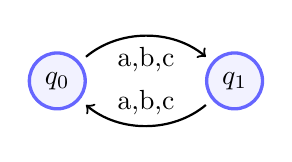
\begin{tikzpicture}[
	state/.style={circle, draw=blue!60, fill=blue!5, very thick, node distance=1.5cm},
	start/.style={name=start},
	input/.style={->, thick, shorten >= 1mm, shorten <= 1mm},
]
	\node[state, start] {\(q_0\)};
	\node[state, right=of start] (odd) {\(q_1\)};

	\draw[input, bend left=40] (start) to node[below] {a,b,c} (odd);
	\draw[input, bend left=40] (odd) to node[above] {a,b,c} (start);
\end{tikzpicture}
\end{document}
